%-------------------------------------------------------------------------------------------
% Vorlage erstellt von sli92
% Latex für Einsteiger: http://latex.mschroeder.net/#textformatierung
% Formeln in Latex: http://www.hosi.de/latex/mathe.htm
%-------------------------------------------------------------------------------------------
%PRÄAMBEL
%-------------------------------------------------------------------------------------------

\documentclass[a4paper,14pt,headsepline]{scrartcl}

\usepackage[ngerman]{babel}
\usepackage[utf8]{inputenc}
\usepackage{fancyheadings}
\usepackage{graphicx}
\usepackage{eurosym}

% Absatzeinrückung
%++++++++++++++++++++++++++
%\setlength{\parskip}{5pt}
%\setlength{\parindent}{0pt}

\setlength{\parskip}{1.5em}
\setlength{\parindent}{0pt}

% Kopf- und Fußzeile
%++++++++++++++++++++++++++

\pagestyle{fancy}
\lhead{\bfseries netcon}
%\chead{Lipp}
\rhead{\nouppercase{\leftmark}}

%C für Center
\fancyfoot[C]{ \thepage}

%-------------------------------------------------------------------------------------------
%DOKUMENT
%-------------------------------------------------------------------------------------------

\begin{document}

% Titelseite
%++++++++++++++++++++++++++
\author{Lipp, Pietryka} 
\title{Diplomarbeit: netcon} 
\date{} 
\maketitle

\newpage

\section*{Zusammenfassung}
\newpage

\section*{Abstract}
\newpage

\section*{Danksagung}
\newpage

\section*{Einleitung}
In vielen Fällen ist bereits eine Infrastruktur vorhanden, sei es ein Firmen- oder. Heimnetzwerk auf Ethernet-Basis. Wieso sollte man dieses nicht nutzen, um einfache Steuer- und Messaufgaben zu realisieren? Wieso müssen für einfachste Anwendungen, wie z.B. die Überwachung von Wettergrößen, bereits neue Messsysteme angeschafft werden? Das dafür notwendige Netzwerk, ist häufig bereits vorhanden. Vor allem Privatanwender wünschen sich oft eine kostengünstige Möglichkeit. Netcon hat das Ziel, diesem Bedürfnis nachzukommen und eine einfache Lösung anzubieten. Zudem stehen alle erstellten Entwicklungen unter der OpenSource-Lizenz. 

Diese Diplomarbeit soll im ersten Teil einen Überblick verschaffen, wie so ein netcon-System in den Grundzügen aufgebaut ist. Danach geht es zum Grundlagen-Kurs, der je nach Bedarf gelesen werden kann um dann die zwei großen Kapitel Hardware und Software zu verstehen.

Viel Spaß!

\newpage

% Inhaltsverzeichnis
%++++++++++++++++++++++++++
\tableofcontents
\newpage

%Inhalt
%++++++++++++++++++++++++++

\section{Überblick}

\subsection{Was ist netcon?}
\textbf{Netcon} bezeichnet ein flexibles Mess- und Steuersystem zur Einbindung in ein bestehendes Ethernet-Netzwerk. 

Das System garantiert kein Echtzeitverhalten, weshalb es auch nur für nicht zeitkritische Anwendungen geeignet ist. Grund hierfür ist die Wahl der Kommunikationsschnittstelle, die mit dem Internet Protocol (IP) über Ethernet, zeitkritische Übertragungen nicht sicherstellt. Die Einbindung in ein bestehendes Firmen- oder Heimnetzwerk ist damit aber umso einfacher. Bis auf die Erstellung von netcon-kompatiblen Modulen ist im einfachsten Fall nur ein handelsüblicher Router erforderlich.

Im Gegensatz zu vielen anderen Systemen ist netcon kein Produktpaket, das so im Geschäftsregal stehen soll, sondern vielmehr eine Vereinbarung bzw. Protokoll, woran sich Aktor- oder Sensormodule halten müssen um gemeinsam in einem System zu funktionieren. Dazu stellt die Diplomarbeit Firmware für einige Mikrocontroller-Systeme und eine plattformunabhängige Verwaltungsumgebung zur Verfügung. 

Im Rahmen dieser Diplomarbeit wurden also netzwerkfähige Steuer- und Messmodule geschaffen, auf die in Kapitel \textbf{Hardware} noch weiter eingegangen wird. Die zentrale Software zur Verwaltung der Module wird in Kapitel \textbf{Software} näher beschrieben. 

Vorher wird der grundlegende Aufbau des netcon-Systems erklärt und benötigte Grundlagen behandelt.

\subsection{Grundlegender Aufbau}
Vorausgesetzt das Netzwerk besteht bereits, sind weiters netzwerkfähige Aktor- und Messmodule, sowie eine Betriebsumgebung für die Verwaltungssoftware notwendig. Diese Umgebung kann jeder Computer sein, der mit einer Java Virtual Runtime und einem httpd-Webserver mit PHP Unterstützung ausgestattet ist. Die Module müssen sich an die Konventionen halten, die in zwei Protokollen spezifiziert sind. Dazu näheres in Kapitel Hardware. Abb. 1 zeigt den grundlegenden Aufbau eines solchen Systems. 

\begin{figure}[h]
\begin{center}
\fbox{
	%Rahmengroesse	
	\begin{minipage}{0.7 \paperwidth}
	\begin{center}
	%Bildgroesse
	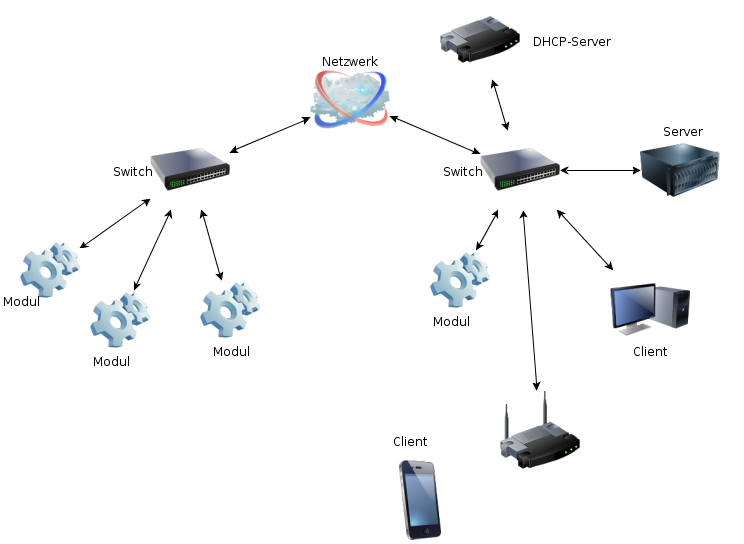
\includegraphics[width=0.7 \paperwidth]{./bilder/netcon_aufbau.png}
	\caption{Grundlegender Aufbau}
	\end{center}
	\end{minipage}
}
\end{center}
\end{figure}

\newpage

Empfehlenswert ist ein DHCP-Server, der sich um die automatische Zuweisung der IP-Adressen im Netzwerk kümmert. Die statische Vergabe ist dennoch möglich. Als Firmenanwender wird dieser DHCP-Server wahrscheinlich ein eigener Computer sein. Privatanwender verwenden im Normalfall einen \linebreak (WLAN)Router. Abb.1 ist auf den Einsatz in Unternehmen ausgerichtet. Privatanwender benötigen oftmals keinen Switch, sondern lediglich ihren bereits vorhandenen 4-Port-Router. Dieses Szenario ist in Abb. 2 verdeutlicht. 

\begin{figure}[h]
\begin{center}
\fbox{
	%Rahmengroesse	
	\begin{minipage}{0.7 \paperwidth}
	\begin{center}
	%Bildgroesse
	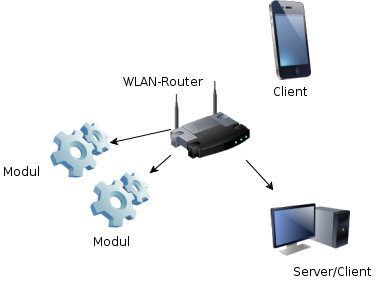
\includegraphics[width=0.5 \paperwidth]{./bilder/netcon_aufbau_privat.png}
	\caption{Grundlegender Aufbau für Privatanwender}
	\end{center}
	\end{minipage}
}
\end{center}
\end{figure}

Die Verwaltungssoftware läuft entweder separat auf einem Server, oder gemeinsam auf dem Client-Computer, auf dem zur Anzeige der Messdaten und zur Steuerung der Aktormodule eine Website aufgerufen wird. 

\newpage

\subsection{Systemvoraussetzungen}

Zusammengefasst sind folgende Komponenten erforderlich:

\begin{itemize}

\item DHCP-Server (z.B. handelsüberlicher Router)
\item Switch (falls mehr Ports erforderlich)
\item Computer/Server (für den Betrieb der Verwaltungssoftware)
\item Netzwerkfähige Aktor- oder Sensormodule mit implementierten netcon-Protokoll\footnote{Im Kapitel Hardware werden Mikrocontroller-Kits vorgestellt, für die bereits Firmware zur Verfügung steht.} 
\item Netzwerkkabel für die Verbindung der Komponenten bzw. Access Point bei drahtloser Übertragung

\end{itemize}

Der Computer/Server sollte folgende Anforderungen  erfüllen:

\begin{itemize}

\item 1 GHz CPU
\item 256 MB RAM (nur für netcon)
\item Netzwerkkarte
\item Betriebssystem inkl. Java JRE 6 und PHP-Webserver
\item SSH-Zugang oder Monitor

\end{itemize}

Je nach Wahl des Betriebssystems können die Anforderungen noch höher, oder sogar schwächer ausfallen.


\newpage
\subsection{Funktionsweise}

\subsubsection{Server}

\textbf{Netcon Server}, die Verwaltungssoftware besteht aus zwei Teilen (siehe Abb. 3). Dem Daemon \textbf{netcond}, zuständig für die Überwachung und Verwaltung der einzelnen Module und Schnittstelle zum Webserver \textbf{netcon web}. Dieser stellt das grafische Frontend bereit, über das Anwender mittles Webbrowser einsteigen können, um sich beispielsweise Messdaten anzeigen zu lassen. 

\begin{figure}[h]
\begin{center}
\fbox{
	%Rahmengroesse	
	\begin{minipage}{0.7 \paperwidth}
	\begin{center}
	%Bildgroesse
	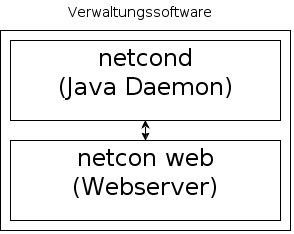
\includegraphics[width=0.4 \paperwidth]{./bilder/netcon_server_aufbau.png}
	\caption{Aufbau von netcon Server}
	\end{center}
	\end{minipage}
}
\end{center}
\end{figure}

Der Daemon sucht nach dem Start alle paar Sekunden das Netzwerk nach verbunden Modulen ab und hält diese in einer Liste. Für jedes dieser Module wird ein neuer Programmfaden erzeugt, der ständig Messdaten abfragt und diese speichert, sowie die Steuerung der Module auf Anfrage übernimmt. Zusätzlich startet der Daemon einen weiteren Prozess, die Schnittstelle, über die der Webserver dann Daten abfragen und Steuerinformationen übermitteln kann. Verbindet sich ein Webbrowser zu diesem Webserver, weißt ein PHP-Script den Daemon an, die aktuellen Daten zu übermitteln. Diese werden dann auf der Website angezeigt. Genau umgekehrt können auch Steuerdaten übermittelt werden z.B. bei Drücken eines Buttons. Dieses Prinzip ist nocheinmal in Abb.4 grafisch verdeutlicht.

\newpage

\begin{figure}[h]
\begin{center}
\fbox{
	%Rahmengroesse	
	\begin{minipage}{0.8 \paperwidth}
	\begin{center}
	%Bildgroesse
	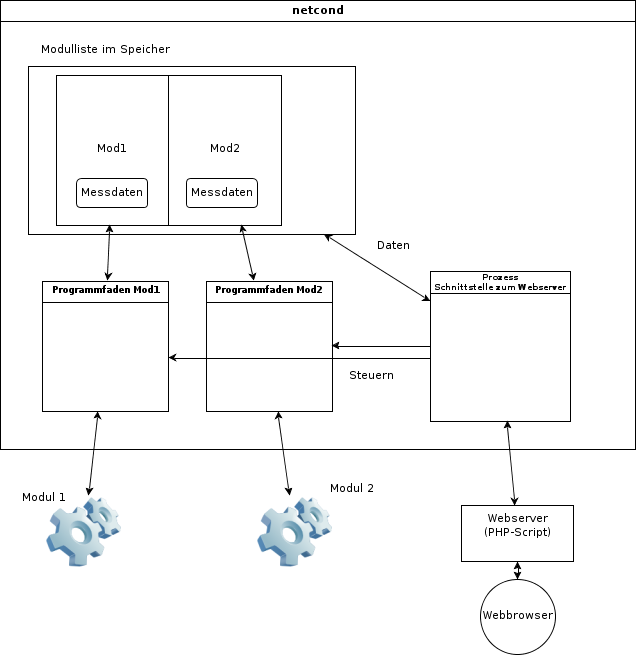
\includegraphics[width=0.7 \paperwidth]{./bilder/netcon_funktionsweise.png}
	\caption{Funktionsweise des Servers}
	\end{center}
	\end{minipage}
}
\end{center}
\end{figure}

Der Webserver kann jeder beliebige http-Server sein, wie z.B. Apache inkl. PHP Integration. Außerdem ist für die Ausführung von netcond eine Java Runtime Environment (JRE) in Version 6 erforderlich. In Kapitel Software wird die Auswahl des Webservers und dessen Konfiguration näher beschrieben. Auch die Installation der Java JRE unter Windows wird erklärt. Andere Betriebssysteme (Mac OS X, Linux) stellen bereits eine bereit.

\newpage

\subsubsection{Module}

Die Module sind Hardware, welche mittels Ethernet über das netcon- Protokoll erreichbar, bedienbar, und abfragbar sind. Sie umfassen Messmodule wie Temperatur-, Luftdruck-, Drehzahlmodule, sowie auch Steuermodule wie Relais- oder Displaymodule. Teilweise sind die Module als LAN-UART Umsetzer konzipiert, um Erstellung eigener Netzwerkfähiger Module zu vereinfachen. Die Module unterstützen das DHCP Protokoll, um sich ohne IP-Konfiguration ins Netzwerk einzubinden.

Grafik Aufbau der Module 

Grundlegende Funktionsweise


\newpage

\section{Grundlagen}

\section{Hardware}
\subsection{Auswahl des Ethernet Controllers}
Damit ein Mikrocontroller über das Ethernet kommunizieren kann, wird eine entsprechende Hardware benötigt, der sogenannte Ethernet Controller. Ein Ethernet Controller übernimmt dabei die Aufgaben der OSI-Schichten 1(Physical) und 2(Data-Link). Der Controller benötigt zudem einen entsprechend großen Empfangspuffer, um mindestens einen vollwertigen Ethernet-Frame(1542 Byte) aufzunehmen zu können. Dabei standen für 8-Bit Mikrocontroller vorerst zwei verschiedene Bausteine zur Auswahl, einmal der CP2200 von SiLabs, und einmal der ENC28J60 von Microchip. Beide Controller haben, was die Netzwerkkommunikation angeht, so ziemlich die selben Features, der gravierende Unterschied liegt jedoch in der Ansteuerung dieser. Der CP2200 wurde von SiLabs, wie es scheint, nur für die Verwendung mit einem Mikrocontroller vom Typ 8051 entwickelt, die Ansteuerung erfolgt deshalb über einen parallelen Adress-/Datenbus wodurch man mindestens 16 Leitungen und Pins am Mikrocontroller benötigt. Beim ENC28J60 erfolgt die Kommunikation über den SPI-Bus, daher benötigt man nur vier Leitungen(MOSI, MISO, SCK, CS), dadurch hat auch der Netzwerkcontroller selber nur 28 Pins und ist auch im "bastlerfreundlichen" DIP-Gehäuse zu bekommen. Ein anderer Faktor für die Auswahl des ENC28J60 war das Vorhandensein einer günstigen Entwicklungsplatine, es gibt bei Pollin den AVR-NET-IO Bausatz, dieser kostet nur \EUR{20} und enthält alle für die Netzwerkprogrammierung benötigten Komponenten(ATmega32, ENC28J60, RJ-45 Buchse).

\subsection{ENC28J60 Beschaltung}
Die Aussenbeschaltung benötigt neben einigen Standardbauelementen auch einige 1\% Widerstände und einen 1:1 Übertrager, jedoch gib es RJ-45 Buchsen in denen bereits der Übertrager, sowie die LEDs bereits eingebaut sind.
\begin{figure}[h]
\begin{center}
\fbox{
	%Rahmengroesse	
	\begin{minipage}{0.7 \paperwidth}
	\begin{center}
	%Bildgroesse
	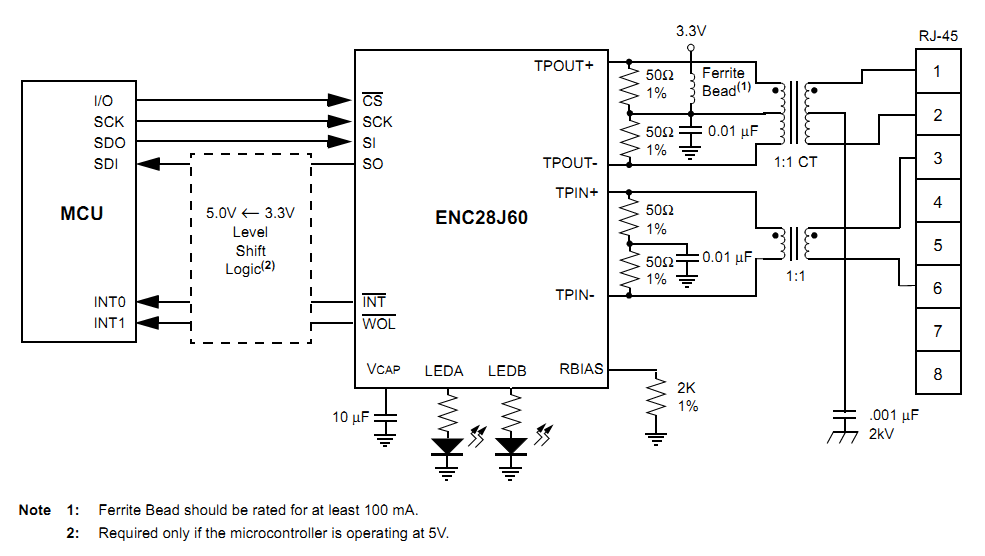
\includegraphics[width=0.7 \paperwidth]{./bilder/enc28j60_beschaltung.png}
	\caption{Aussenbeschaltung ENC28J60}
	\end{center}
	\end{minipage}
}
\end{center}
\end{figure}



\subsection{ENC28J60 Treibersoftware}

\section{Software}

 
\end{document}